\documentclass[border=10pt,tikz]{standalone}
\usepackage{tikz}
\usetikzlibrary{positioning,arrows.meta,shapes,fit,backgrounds}

\begin{document}
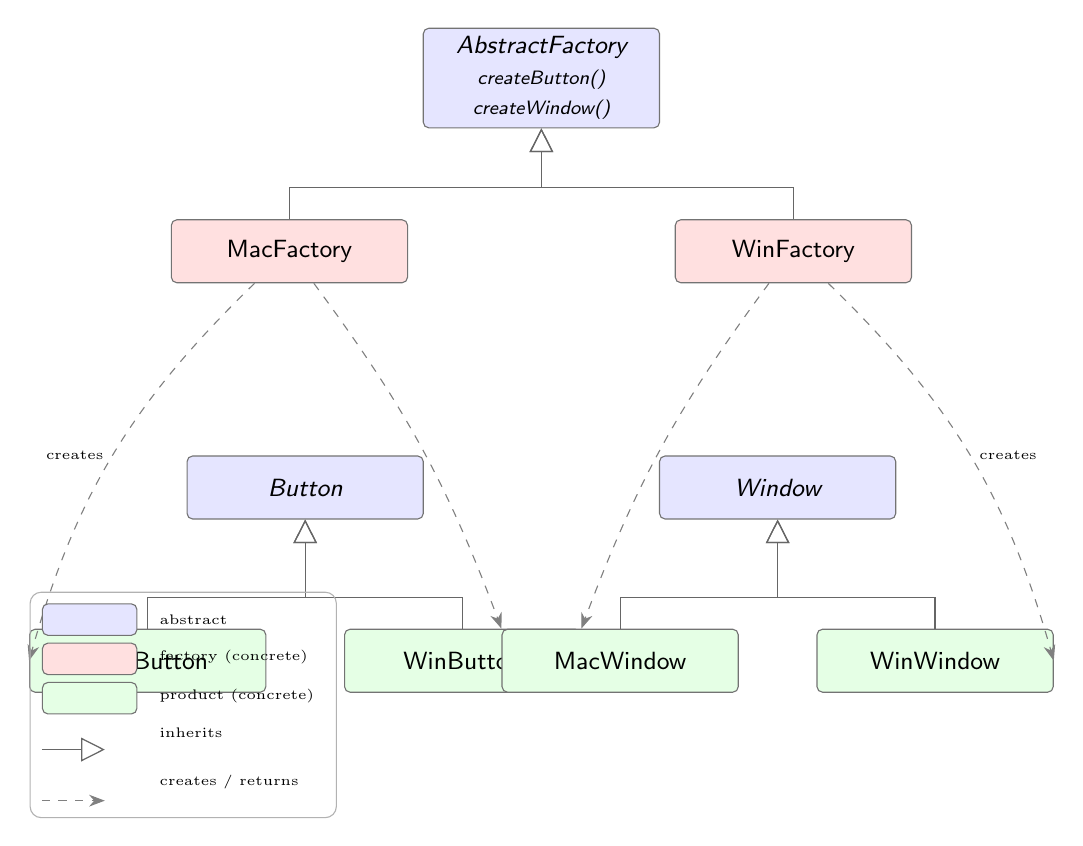
\begin{tikzpicture}[
  font=\sffamily\small,
  cls/.style={
    rectangle, rounded corners=2pt,
    draw=black!55, line width=0.4pt,
    minimum height=8mm, minimum width=30mm,
    inner sep=3pt, fill=white,
    align=center
  },
  abs/.style={cls, fill=blue!10, font=\sffamily\itshape\small},
  fac/.style={cls, fill=red!12},
  pro/.style={cls, fill=green!10},
  inh/.style={
    -{Triangle[length=3mm,width=3mm,open]},
    draw=black!60, line width=0.45pt
  },
  ret/.style={
    -{Stealth[length=2mm]}, dashed,
    draw=black!50, line width=0.4pt
  },
  group/.style={
    rectangle, rounded corners,
    draw=black!25, dotted, line width=0.4pt,
    inner sep=6pt, inner ysep=8pt
  }
]

% ─── Factory layer ──────────────────────────────────────────
\node[abs] (af) at (0, 4) {AbstractFactory \\ \scriptsize createButton() \\ \scriptsize createWindow()};

\node[fac] (mf) at (-3.2, 1.8) {MacFactory};
\node[fac] (wf) at ( 3.2, 1.8) {WinFactory};

\draw[inh] (mf.north) -- ++(0,0.4) -| (af.south);
\draw[inh] (wf.north) -- ++(0,0.4) -| (af.south);

% ─── Product layer ──────────────────────────────────────────
\node[abs] (btn) at (-3, -1.2) {Button};
\node[abs] (win) at ( 3, -1.2) {Window};

\node[pro] (mb)  at (-5, -3.4) {MacButton};
\node[pro] (wb)  at (-1, -3.4) {WinButton};
\node[pro] (mw)  at ( 1, -3.4) {MacWindow};
\node[pro] (ww)  at ( 5, -3.4) {WinWindow};

\draw[inh] (mb.north) -- ++(0,0.4) -| (btn.south);
\draw[inh] (wb.north) -- ++(0,0.4) -| (btn.south);
\draw[inh] (mw.north) -- ++(0,0.4) -| (win.south);
\draw[inh] (ww.north) -- ++(0,0.4) -| (win.south);

% ─── Returns (factory → product) ────────────────────────────
\draw[ret] (mf) to[bend right=15] node[left,font=\tiny]{creates} (mb.west);
\draw[ret] (mf) to[bend left=8]  (mw.north west);
\draw[ret] (wf) to[bend left=15] node[right,font=\tiny]{creates} (ww.east);
\draw[ret] (wf) to[bend right=8] (wb.north east);

% ─── Legend ─────────────────────────────────────────────────
\matrix[
  draw=black!30, rounded corners, inner sep=4pt,
  row sep=1pt, column sep=4pt,
  font=\tiny, anchor=south west
] at (-6.5, -5.4) {
  \node[abs, minimum width=12mm, minimum height=4mm]{}; & \node{abstract}; \\
  \node[fac, minimum width=12mm, minimum height=4mm]{}; & \node{factory (concrete)}; \\
  \node[pro, minimum width=12mm, minimum height=4mm]{}; & \node{product (concrete)}; \\
  \draw[inh] (0,0) -- (8mm,0); & \node{inherits}; \\
  \draw[ret] (0,0) -- (8mm,0); & \node{creates / returns}; \\
};

\end{tikzpicture}
\end{document}
